\documentclass[11pt,a4paper]{article}
\usepackage[T1]{fontenc}
\usepackage[utf8]{inputenc}
\usepackage{lmodern,microtype}
\usepackage{amsmath,amssymb,amsthm,mathtools,bm}
\usepackage{booktabs,array,tabularx,longtable}
\usepackage{graphicx,float,caption}
\usepackage{xcolor}
\usepackage[margin=22mm]{geometry}
\usepackage{enumitem}
\usepackage{fancyhdr}
\usepackage[hidelinks]{hyperref}
\hypersetup{
  pdftitle={FIN Programs P527-P536: Auxiliary-Field Source, Memory Realization, and Independent Exact Replay},
  pdfauthor={Krzysztof Żuchowski},
  pdfsubject={Minimal nonlinear source, nonlinear orbital audit, temporal-memory classification, exact FFT and PSD certificates, inverse observability},
  pdfkeywords={FIN, DNLS, auxiliary field, Schur complement, orbital stability, memory kernel, recurrence, interval FFT, PSD, identifiability}
}
\setlength{\parindent}{0pt}
\setlength{\parskip}{0.55em}
\setlength{\headheight}{14pt}
\setlist[itemize]{leftmargin=1.6em,itemsep=0.2em,topsep=0.2em}
\pagestyle{fancy}
\fancyhf{}
\lhead{FIN Programs P527--P536}
\rhead{Release 10.53}
\cfoot{\thepage}
\newtheorem{theorem}{Theorem}[section]
\newtheorem{proposition}[theorem]{Proposition}
\newtheorem{corollary}[theorem]{Corollary}
\newcommand{\proven}{\textcolor{green!50!black}{\textbf{[PROVEN]}}}
\newcommand{\strong}{\textcolor{blue!70!black}{\textbf{[STRONG EVIDENCE]}}}
\newcommand{\conditional}{\textcolor{black!60}{\textbf{[CONDITIONAL]}}}
\newcommand{\moderate}{\textcolor{orange!85!black}{\textbf{[MODERATE EVIDENCE]}}}
\newcommand{\refuted}{\textcolor{red!75!black}{\textbf{[REFUTED CANDIDATE]}}}
\newcommand{\claimbox}[1]{\begin{center}\fcolorbox{blue!60!black}{blue!4}{\parbox{0.91\textwidth}{#1}}\end{center}}

\begin{document}

\pagenumbering{gobble}
\begin{titlepage}
\centering
\vspace*{1.8cm}
{\LARGE\bfseries FIN Programs P527--P536\par}
\vspace{0.7cm}
{\Large Auxiliary-Field Source, Memory-Realization Dependence,\par and Independent Exact Replay\par}
\vspace{0.5cm}
{\large Ten local analytical and computational studies following Release 10.52\par}
\vspace{1.5cm}
{\Large Krzysztof Żuchowski\par}
\vspace{0.3cm}
{\large Independent Researcher --- Fractal Information Theory Project\par}
{\large ORCID: 0009-0002-0909-3613\par}
\vspace{1.3cm}
{\large FIN Release 10.53 --- Version 1.0.0\par}
{\large 10 August 2026\par}
\vfill
\begin{minipage}{0.84\textwidth}
\textbf{Scope.} This report executes P527--P536. It constructs the smallest auxiliary-field mechanism that forces the missing attractive fourth-order jet, checks nonlinear dynamics on both sides of the certified VK boundary, and distinguishes static from temporal memory realization. It also replaces two upstream numerical trust assumptions with independently replayable certificates.\par
\textbf{Evidence boundary.} Exact finite algebra, exact rational replay, outward disk arithmetic, conservation-controlled finite dynamics, and synthetic operational specifications are admitted. No laboratory evidence, external audit, dimensional calibration, or particle identification is asserted.\par
\textbf{Reproduction.} The deterministic research batch ran locally in approximately 65.7 seconds. Eleven acceptance tests passed; three exported certificate families passed standard-library replay.\par
\textbf{Repository.} \url{https://github.com/hyconiek/Fractal-Nadsoliton-Theory}\par
\textbf{License.} CC BY 4.0.
\end{minipage}
\end{titlepage}
\pagenumbering{arabic}

\begin{abstract}
P527 finds a smallest conditional mechanism for the focusing nonlinearity that earlier information-function searches could not select. Let a positive auxiliary mediator have energy
\[
 E(\chi,\rho)=\tfrac12\langle\chi,B\chi\rangle-g\langle\chi,\rho\rangle,
 \qquad B>0,\qquad \rho_x=|\psi_x|^2.
\]
Stationary elimination gives
\[
 E_{\rm eff}(\rho)=-\tfrac{g^2}{2}\langle\rho,B^{-1}\rho\rangle.
\]
For $B=bI$, this is precisely an attractive local quartic. Positivity of $B$, a nonzero linear density coupling, and stationary elimination are individually necessary for this one-field sign mechanism. The construction is a genuine mathematical bridge candidate, but FIN does not yet source the mediator, $g^2/b$, or the higher-order stabilization required for global boundedness.

P528 exactly replays the 208 state charts and 207 interface boxes of the O223 stability tube. P529 then evolves perturbed stationary states with norm-preserving Strang splitting. The stable-side cases $\omega=0.75,1.00$ remain within orbital distance $0.0053$ to time $80$, whereas $\omega=0.70$ reaches $0.199$ at the finest step and has positive linearized growth rate $0.2256$. This is strong numerical support for the certified VK separation, not an interval enclosure of the nonlinear flow.

P530 gives a decisive nonuniqueness result for memory. Relaxational and Hamiltonian hidden-variable realizations can have the same zero-frequency Stieltjes operator while possessing different temporal spectra. The relaxation family remains unstable over six decades of relaxation time. At full loading, the Hamiltonian realization becomes numerically spectrally stable above mediator speed about $1.585$. Hence a static memory operator does not determine a temporal law or its stability.

P531 proves that no exact linearly translating recurrence with inverse participation ratio above $1/8$ exists for the strict linear flow; a 13-kick nonlinear search finds no relative-periodic candidate. P532 turns the six-frequency independence theorem into quantitative dimensionless recurrence bounds and finds integer time $1{,}752{,}344$ with phase sup-error $0.14604$. No absolute time unit follows.

P533 replaces P523's declared FFT envelope by outward centre--radius transforms paying input, twiddle, butterfly and summation errors. The certified $C_{384}$-to-limit fingerprint bound is at most $0.065075$. P534 independently rebuilds all 573 PSD classifications from Machin/atanh constants, Taylor transcendental bounds, exact rational signs, and local subdivision; every class agrees with P514. P535 inverts the detector polytope into explicit synthetic tolerance caps and a raw-event schema. P536 proves that finite-record law inference remains prior-conditioned: likelihood is constant along every vanishing-bump fiber, so the posterior along that fiber is inherited from the prior.

The main scientific advance is therefore not a physical closure. It is a sharper separation of obligations: a minimal attractive-response mechanism now exists; the localized branch and its stable sector survive direct nonlinear testing; static memory does not select dynamics; and two major numerical ledgers have independent certificate layers. The mediator's FIN-internal origin, dimensional scale, selector, and experimental realization remain open.
\end{abstract}

\textbf{Status vocabulary.} \proven{} denotes an analytic theorem or exact/outward finite certificate in its declared model; \strong{} denotes robust finite numerical evidence; \conditional{} marks an added mediator, law, operational budget or prior; \moderate{} denotes bounded incomplete evidence; \refuted{} denotes failure of a precisely stated candidate.

\tableofcontents
\newpage

\section{Executive result map}

\claimbox{\textbf{Central result.} A positive quadratic mediator linearly coupled to information density supplies the attractive quartic sign by a Schur complement. This is the smallest mechanism found so far that repairs the fourth-jet obstruction. It is not yet a derivation from FIN: the mediator, coupling scale and saturation law are new typed premises.}

\begin{longtable}{@{}p{0.065\textwidth}p{0.22\textwidth}p{0.43\textwidth}p{0.20\textwidth}@{}}
\caption{Programs, generated objects and verdicts.}\\
\toprule
ID & Generated object & Main result & Status\\
\midrule
\endfirsthead
\toprule
ID & Generated object & Main result & Status\\
\midrule
\endhead
P527 & O231 positive-mediator source & Positive mediator elimination forces an attractive local or nonlocal quartic; its magnitude and origin remain free. & \proven{} / \conditional\\
P528 & O232 exact O223 replay & All 208 charts and 207 bridges pass exact dyadic-rational acceptance replay. & \proven\\
P529 & O233 orbital dynamics audit & Stable-side perturbations remain localized; the negative-VK case grows. & \strong{} / \conditional\\
P530 & O234 realization classification & One static memory operator admits temporally inequivalent stable/unstable realizations. & \strong{} / \proven{} no-inference\\
P531 & O235 translation obstruction & Exact linear localized translation is impossible above IPR $1/8$; no nonlinear candidate appears in the scan. & \proven{} / \strong\\
P532 & O236 six-torus recurrence & Equidistribution and Dirichlet recurrence are quantitative, but remain dimensionless. & \proven\\
P533 & O237 outward FFT certificate & All FFT rounding is paid explicitly; maximum $C_{384}$-limit bound is $0.065075$. & \proven{} / computer-assisted\\
P534 & O238 independent PSD audit & An independent rational-transcendental engine reproduces all 573 P514 classes. & \proven\\
P535 & O239 inverse detector envelope & A maximum-product error allocation and raw-event schema are produced. & \conditional\\
P536 & O240 prior-fiber theorem & Finite records identify a law-equivalence class, not a prior-free law. & \proven\\
\bottomrule
\end{longtable}

\section{Shared mathematical model and noninheritance rules}

The strict working matrix is the finite circulant graph operator
\[
 W_{xy}=\frac{\cos(0.18575d(x,y)+0.16250)}{1+d(x,y)^{9/5}},
 \qquad A=\operatorname{diag}(W\mathbf1)-W\succeq0,
\]
on $\mathbb Z/12\mathbb Z$. The nonlinear equation under audit is
\begin{equation}
 i\dot\psi=A\psi-|\psi|^2\psi,
 \qquad Au+\omega u-u^{\circ3}=0.                 \label{eq:dnls53}
\end{equation}
after the standard rotating-frame convention.

Equation \eqref{eq:dnls53} is not a consequence of $A$ alone. The strict kernel supplies a quadratic generator. P527 supplies a candidate mechanism for the missing nonlinear sign only after a mediator sector is appended. Likewise, the historical legacy kernel remains an intermediate bridge object; no electromagnetic, Planck, hierarchy, gravity, matter or other legacy physical role is transferred to the strict kernel here.

All frequencies and recurrence times are dimensionless. The selector obstruction QW-2191, canonical orientation, laboratory preparation, calibrated clock, apparatus, independent event record and SI conversion remain unsolved.

\section{P527 --- the smallest attractive auxiliary-field mechanism}

\subsection{Invariant fourth-order classification}

For a complex field on twelve sites, global $U(1)$ and site-permutation invariance allow two quartic invariants,
\[
 a\left(\sum_x|\psi_x|^2\right)^2+b\sum_x|\psi_x|^4.
\]
If an energy is additive on fields with disjoint supports, the first term is excluded because it creates cross-support products. The local invariant quartic space is then a single ray, but its coefficient can have either sign. Symmetry classifies the shape; it does not select attraction.

\subsection{Schur-complement construction}

Introduce a real auxiliary field $\chi$ and the information density $\rho_x=|\psi_x|^2$. Set
\begin{equation}
 E_{\rm med}(\chi,\rho)=\frac12\langle\chi,B\chi\rangle-g\langle\chi,\rho\rangle,
 \qquad B=B^*>0.                                  \label{eq:mediator}
\end{equation}
The stationary equation is $B\chi=g\rho$, hence $\chi_*=gB^{-1}\rho$. Substitution gives
\begin{equation}
 E_{\rm med}(\chi_*,\rho)=-\frac{g^2}{2}\langle\rho,B^{-1}\rho\rangle\le0. \label{eq:schur}
\end{equation}
For $B=bI$,
\[
 E_{\rm med}^{\rm eff}=-\frac{g^2}{2b}\sum_x|\psi_x|^4,
\]
which yields the focusing cubic response in the Euler--Lagrange equation. For general positive $B$, the same sign is forced but the response is nonlocal.

\begin{theorem}[Minimal sign-forcing mediator]
Within the declared quadratic-mediator/linear-density-coupling mechanism, the following are sufficient and individually necessary to generate a closed attractive quartic after elimination: (i) a positive mediator quadratic form, (ii) a nonzero linear coupling to $\rho=|\psi|^2$, and (iii) stationary or adiabatic elimination of the mediator. Locality $B=bI$ is necessary only if an onsite rather than nonlocal quartic is required.
\end{theorem}

Removing positivity loses existence and sign control of the minimizing mediator. Removing the coupling yields no quartic. Removing elimination leaves a two-field temporal system rather than the one-field DNLS. Removing locality retains attraction but changes its spatial form.

\textbf{Unpaid obligations.}
\begin{itemize}
\item The ratio $g^2/b$ is not determined by the strict spectrum or information language.
\item Equation \eqref{eq:schur} is unbounded below as a global large-density energy unless a saturating or higher-order positive response is retained.
\item No current strict-core object has been shown to be $\chi$ or $B$.
\item A temporal mediator requires its own kinetic law; P530 shows why its zero-frequency elimination is insufficient.
\end{itemize}

Thus P527 constructs a minimal missing object, not a FIN-internal source theorem.

\section{P528--P529 --- exact stability replay and nonlinear trajectory test}

\subsection{Exact replay of O223}

P528 regenerates the full P519 tube: 208 state boxes cover $0.68\le\omega\le1.20$, and 207 point boxes are nested at their shared boundaries. Every exported hexadecimal binary64 endpoint is converted to an exact dyadic rational. The checker verifies positive Krawczyk margins, defects below one, finite $L_-/L_+$ inertia signs, slope enclosures, curvature enclosures and bridge nesting.

The minimum state inclusion margin is $2.515\times10^{-5}$; the largest defect is $0.006258$; the minimum bridge nesting margin is $6.237\times10^{-5}$. On $[0.70,0.75]$, the minimum exported lower curvature bound is $3.56036$. The accepted transition bracket remains
\[
 [0.722143668857225,\ 0.722143708857225].
\]

\textbf{Trust boundary.} Exact replay validates the accepted inequalities. The upstream generation of the outward state and spectral boxes remains a separate implementation layer.

\subsection{Conservation-controlled nonlinear evolution}

P529 perturbs the site-centred stationary solution by $0.5\%$ in a norm-orthogonal random direction, then applies Strang splitting,
\[
 e^{-i\Delta t A/2}\,e^{i\Delta t|\psi|^2}\,e^{-i\Delta t A/2},
\]
at $\Delta t=0.02,0.01,0.005$ to $T=80$. The method preserves power exactly in exact arithmetic. Orbital distance minimizes over global phase and all twelve translations.

At the finest step, the maximum orbital distances are approximately
\[
 d_{\rm orb}^{\max}(0.70)=0.1991,\qquad
 d_{\rm orb}^{\max}(0.75)=0.00523,\qquad
 d_{\rm orb}^{\max}(1.00)=0.00510.
\]
The corresponding linearized spectral abscissae are $0.22556$, $1.12\times10^{-7}$ and $3.33\times10^{-16}$. Power drift stays below $5.1\times10^{-11}$.

The unstable case is quantitatively step-sensitive because exponential growth amplifies phase error over long time. It is therefore retained as strong evidence rather than promoted to a validated-flow theorem. The stable cases show systematic refinement and remain close to their symmetry orbit.

\begin{figure}[H]
\centering
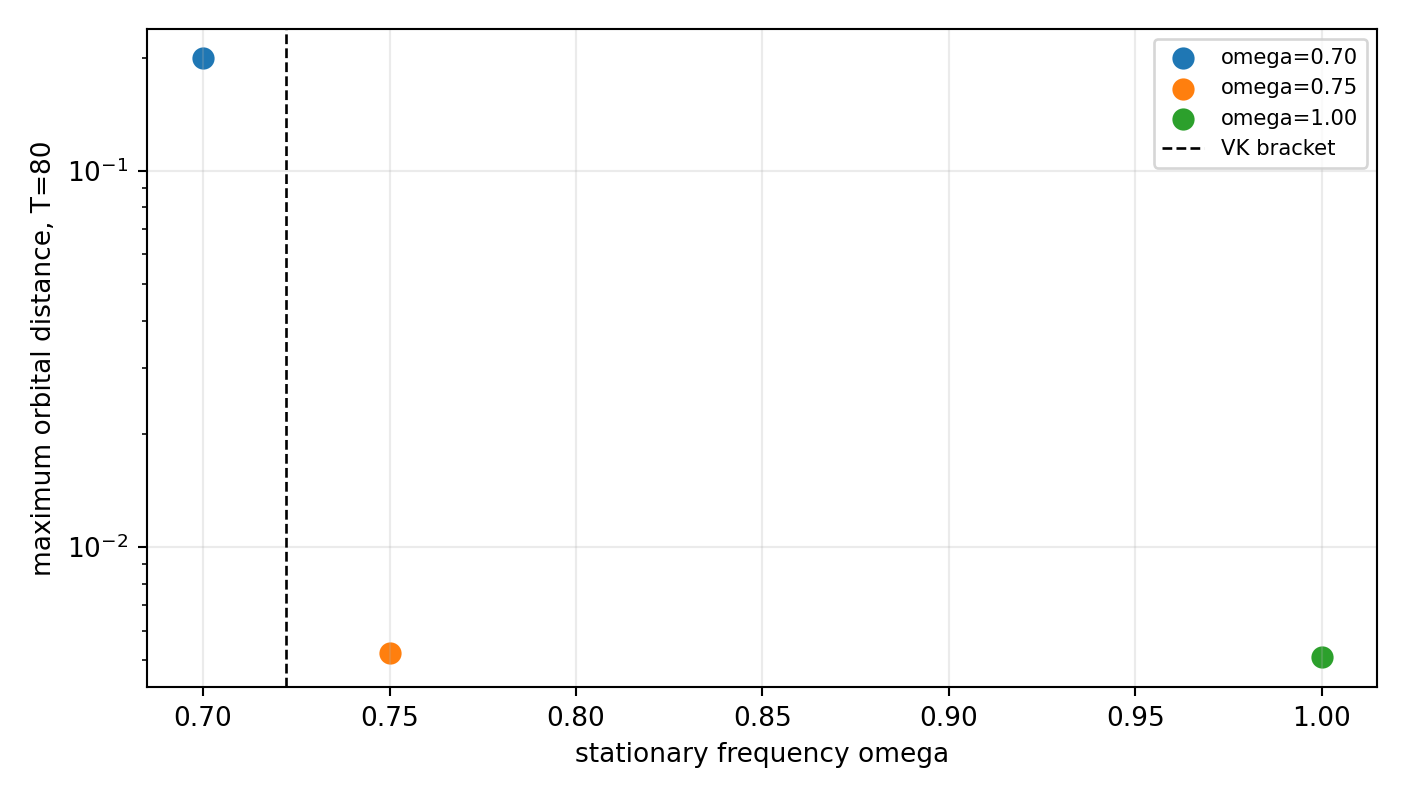
\includegraphics[width=0.78\textwidth]{FIN_Programs_527_536_Figures/p529_orbital_stability.png}
\caption{The direct nonlinear audit separates the negative-VK case from the two favourable-sector cases.}
\end{figure}

\section{P530 --- one static memory, inequivalent temporal laws}

The zero-frequency Stieltjes response is
\[
 M=\sigma(0)I-\sum_j r_j(A+c_jI)^{-1},\qquad c_j,r_j>0.
\]
It fixes a stationary correction but not a unique evolution. P530 compares two explicit hidden-variable classes that reproduce the same static resolvents.

The first is the relaxation class inherited from P521,
\[
 \dot y_j=\tau^{-1}\bigl(\psi-(A+c_jI)y_j\bigr).
\]
Over $10^{-3}\le\tau\le10^3$, every one of 25 finite spectra contains a positive-real-part mode. The maximum spectral abscissa is $1.1244$.

The second class uses Hamiltonian oscillator pairs $(a_j,b_j)$ and a speed parameter $\nu$. Couplings are scaled as $\sqrt{\varepsilon\nu r_j}$ so that stationary elimination retains the declared zero-frequency response. At full loading, the finite scan has unstable spectra at slow speed, including spectral abscissa $0.37785$ at $\nu=1$, but all 19 sampled speeds from $\nu\approx1.585$ through $100$ have real parts below the $2\times10^{-6}$ numerical instability threshold. At $\nu=10$, the residual abscissa is $1.15\times10^{-14}$.

\begin{proposition}[Static-memory underdetermination]
Equality of a zero-frequency memory operator does not imply equality of the augmented temporal generator, its spectral stability, causality realization, dissipation or fluctuation structure. Therefore no temporal stability statement can be inherited from $M$ alone.
\end{proposition}

The proposition is analytic at the level of model nonuniqueness; the location of the Hamiltonian stability boundary is finite numerical evidence. A proof-grade continuation requires Krein-signature and collision analysis.

\begin{figure}[H]
\centering
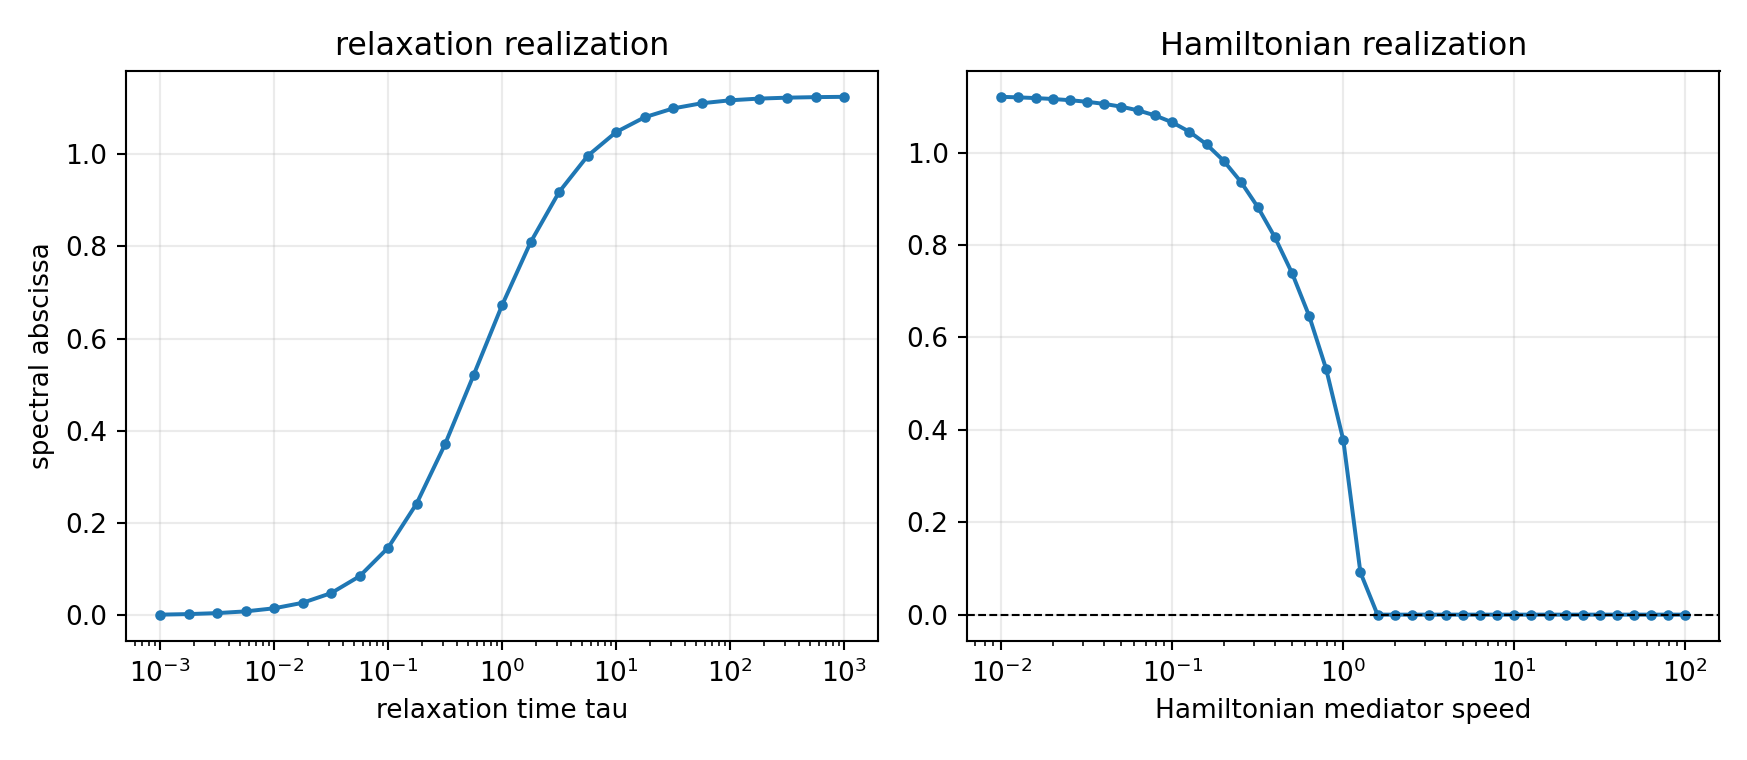
\includegraphics[width=0.94\textwidth]{FIN_Programs_527_536_Figures/p530_memory_realization_dependence.png}
\caption{The same static Stieltjes response supports distinct temporal spectra when embedded in relaxation or Hamiltonian hidden variables.}
\end{figure}

\section{P531 --- translation-resonance obstruction}

Let $S$ be the one-site translation and suppose the linear flow satisfies
\[
 e^{-iTA}\psi=e^{i\theta}S^k\psi.
\]
For every occupied Fourier mode $m$,
\[
 T\lambda_m+\theta+\frac{2\pi km}{12}\in2\pi\mathbb Z.
\]
Subtracting three such equations makes a ratio of two frequency differences rational. P522 excludes this for three distinct nondegenerate strict frequencies. Hence any exact linearly translating recurrence is supported on at most two Fourier modes.

For a normalized vector supported on two conjugate Fourier modes, direct optimization gives
\[
 \operatorname{IPR}(\psi)=\sum_x|\psi_x|^4\le\frac{3}{2N}=\frac18.
\]

\begin{theorem}[Localized linear translation no-go]
The strict linear flow has no exact relative recurrence that translates by a nontrivial lattice shift and has IPR greater than $1/8$.
\end{theorem}

The nonlinear search uses 13 phase kicks from $0.2$ to $1.4$, $\Delta t=0.01$, and $T=300$. Its best one-site phase-matched residual is $0.49458$ at kick $0.5$, even though the state remains localized with IPR $0.6822$. No trial meets the preregistered residual $10^{-3}$ and IPR $0.25$ criteria.

This is a strong finite no-candidate result, not a theorem excluding every nonlinear travelling breather.

\begin{figure}[H]
\centering
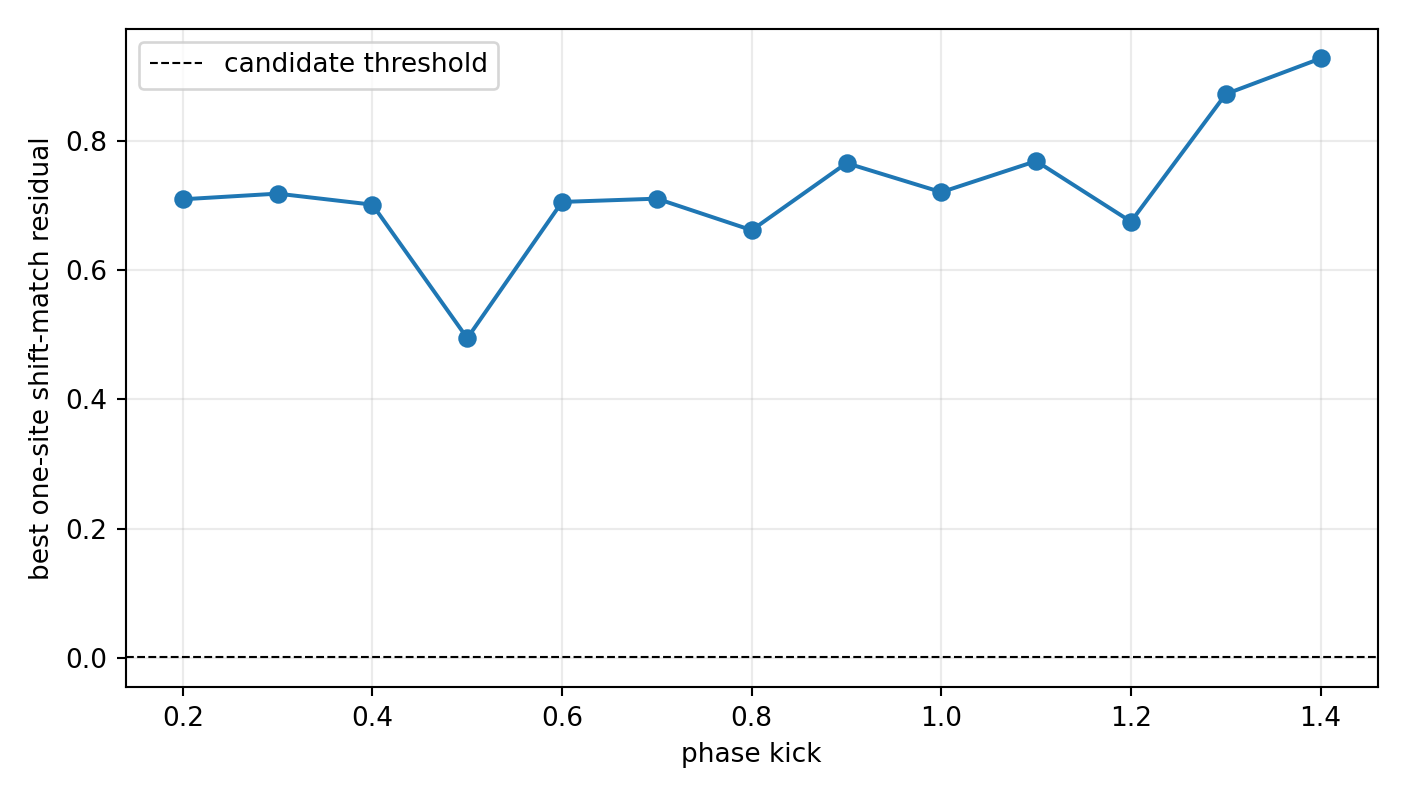
\includegraphics[width=0.78\textwidth]{FIN_Programs_527_536_Figures/p531_translation_scan.png}
\caption{No scanned nonlinear phase kick approaches a one-site relative recurrence.}
\end{figure}

\section{P532 --- quantitative recurrence without an absolute clock}

P522 proved rational independence of the six distinct positive frequencies. Kronecker--Weyl therefore gives unique ergodicity and equidistribution of
\[
 t\longmapsto(t\lambda_1,\ldots,t\lambda_6)\pmod{2\pi}
\]
on $\mathbb T^6$. Dirichlet simultaneous approximation gives, for every integer $Q\ge2$, an integer $1\le q\le Q^6$ whose phase sup-error is at most $2\pi/Q$.

The direct integer scan through $2\times10^6$ finds
\[
 q=1{,}752{,}344,\qquad
 \max_m\operatorname{dist}(q\lambda_m,2\pi\mathbb Z)=0.1460418407.
\]
This is a useful intrinsic recurrence estimate. It cannot be read as seconds: under $A\mapsto cA$, every such time rescales as $q\mapsto q/c$. Soliton frequency can order phase and provide a dimensionless internal clock coordinate, but cannot by itself select an absolute duration.

\section{P533 --- outward FFT certificate}

P523 retained one declared $2\times10^{-9}$ allowance for finite FFT rounding. P533 removes that standalone premise. It encloses every attenuation value and Fourier twiddle using 55-digit reference arithmetic converted to binary64 centre--radius disks. Every radix-two product and butterfly pays input radius, twiddle radius and IEEE-754 operation error. The non-power-of-two $C_{384}$ calculation uses an outward direct DFT.

For the seven resolvent scales
\[
 u\in\{1/8,1/4,1/2,1,2,4,8\},
\]
the minimum response denominator is $2.06676$. The largest transform disk radius is $4.68\times10^{-12}$ for $C_{384}$ and $3.14\times10^{-9}$ at the $262{,}144$-cycle anchor. The analytic Wiener tail then yields the normalized $C_{384}$-to-limit bounds
\[
 (0.065075,0.056464,0.044626,0.032424,0.021061,0.012357,0.006759).
\]

The maximum bound improves from P523's $0.06708$ to $0.065075$ while making the transform error operationally replayable. This remains a computer-assisted proof under the stated floating-point model, not a closed-form limit evaluation.

\begin{figure}[H]
\centering
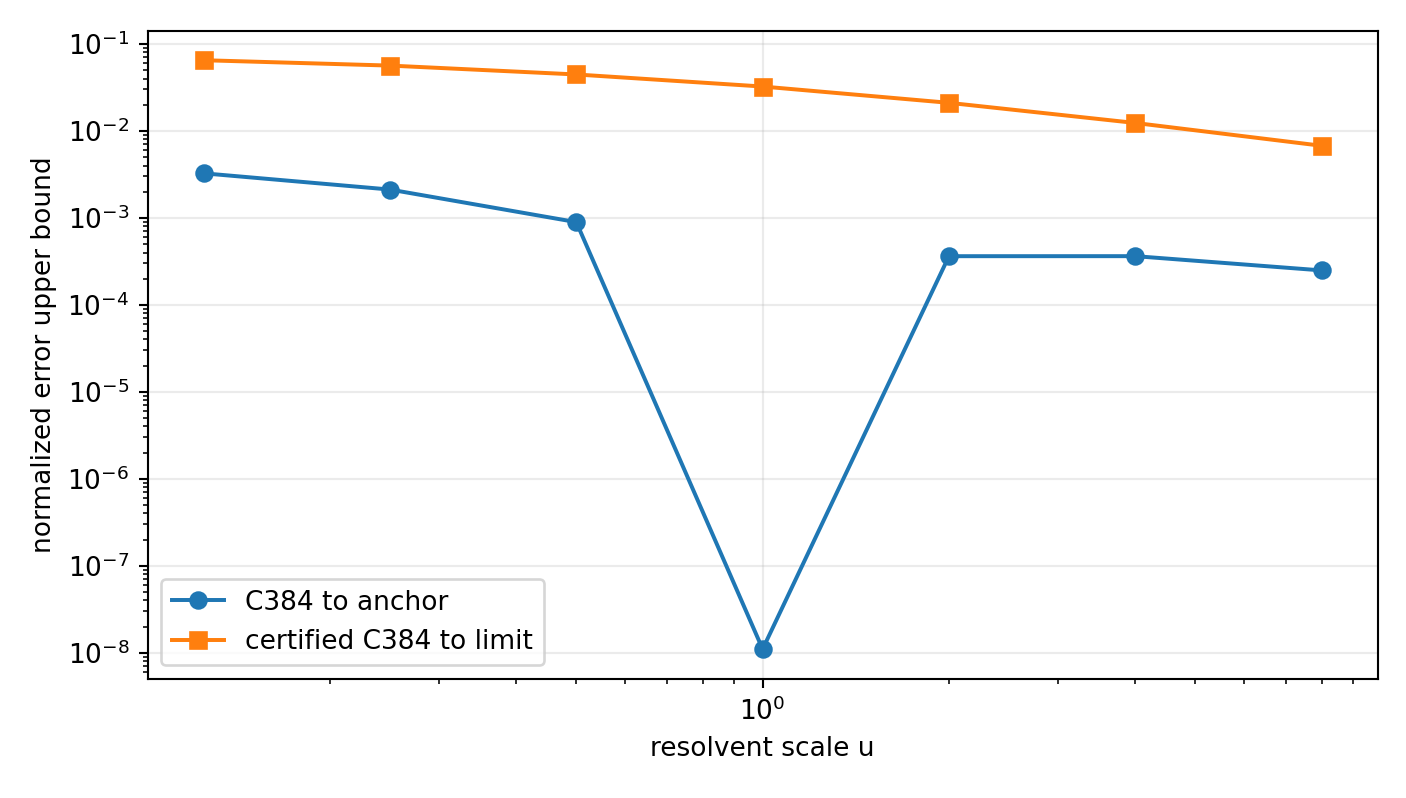
\includegraphics[width=0.78\textwidth]{FIN_Programs_527_536_Figures/p533_outward_fft_bound.png}
\caption{Finite coarse-to-anchor discrepancy and the complete outward $C_{384}$-to-limit certificate.}
\end{figure}

\section{P534 --- an independent rational PSD engine}

P524 replayed P514's exported signs exactly but trusted its upstream transcendental intervals. P534 builds a second route:
\begin{itemize}
\item Machin's formula and alternating arctangent series enclose $\pi$ exactly as rational endpoints;
\item the atanh series encloses $\log d$ for $d=2,\ldots,6$;
\item 78-digit decimal Taylor series with explicit remainder and $10^{-65}$ outward padding enclose exponentials and cosines;
\item exact rational endpoint signs classify each circulant eigenvalue;
\item unresolved wide boxes are subdivided into at most 128 rational subboxes.
\end{itemize}

The engine does not call \texttt{mpmath.iv}, and it does not reuse any P514 eigenvalue endpoint. It reproduces all 573 terminal classes exactly: 388 NONPSD, 182 PSD and 3 unresolved boxes forming the same narrow transition component. No opposite-sign classification occurs.

\begin{theorem}[Independent PSD re-verification]
Within the declared strict-to-positive homotopy and exact decimal parameter convention, all P514 terminal box classifications survive a second, independently generated rational-transcendental enclosure.
\end{theorem}

This materially reduces the probability that the PSD boundary is an artifact of one interval library. It does not give a physical interpolation law or transfer legacy roles.

\section{P535 --- inverse detector envelope}

P525 expressed robust separation as half-spaces
\[
 \sum_{j=1}^7 a_{ij}\varepsilon_j<d_i,
\]
one for each pair of four synthetic dynamics. P535 maximizes $\prod_j\varepsilon_j$ over this positive polytope and recommends $80\%$ of the maximizing coordinates. The resulting caps are:

\begin{center}
\begin{tabular}{lr}
\toprule
Error coordinate & Recommended cap\\
\midrule
loss fraction & 0.114286\\
dark mixture & 0.114286\\
nearest-neighbour coarse graining & 0.104762\\
preparation trace distance & 0.0134413\\
POVM total variation & 0.0134413\\
absolute dimensionless time error & 0.00419755\\
configuration drift TV & 0.0134413\\
\bottomrule
\end{tabular}
\end{center}

The active limiting pair is dephasing versus revival. The conservative point retains minimum pairwise TV lower bound $0.0470446$. A simple union/Hoeffding illustration gives $25{,}629$ events per configuration for $99\%$ simultaneous confidence when the sampling tolerance is one quarter of that margin.

The raw-event schema is
\[
 (\text{timestamp, vertex, preparation, measurement, configuration, run, outcome, custody hash}).
\]
Custody remains provider $\ne$ registrar $\ne$ analyst, hash-before-unblinding, frozen hold-out and one analysis run.

\begin{figure}[H]
\centering
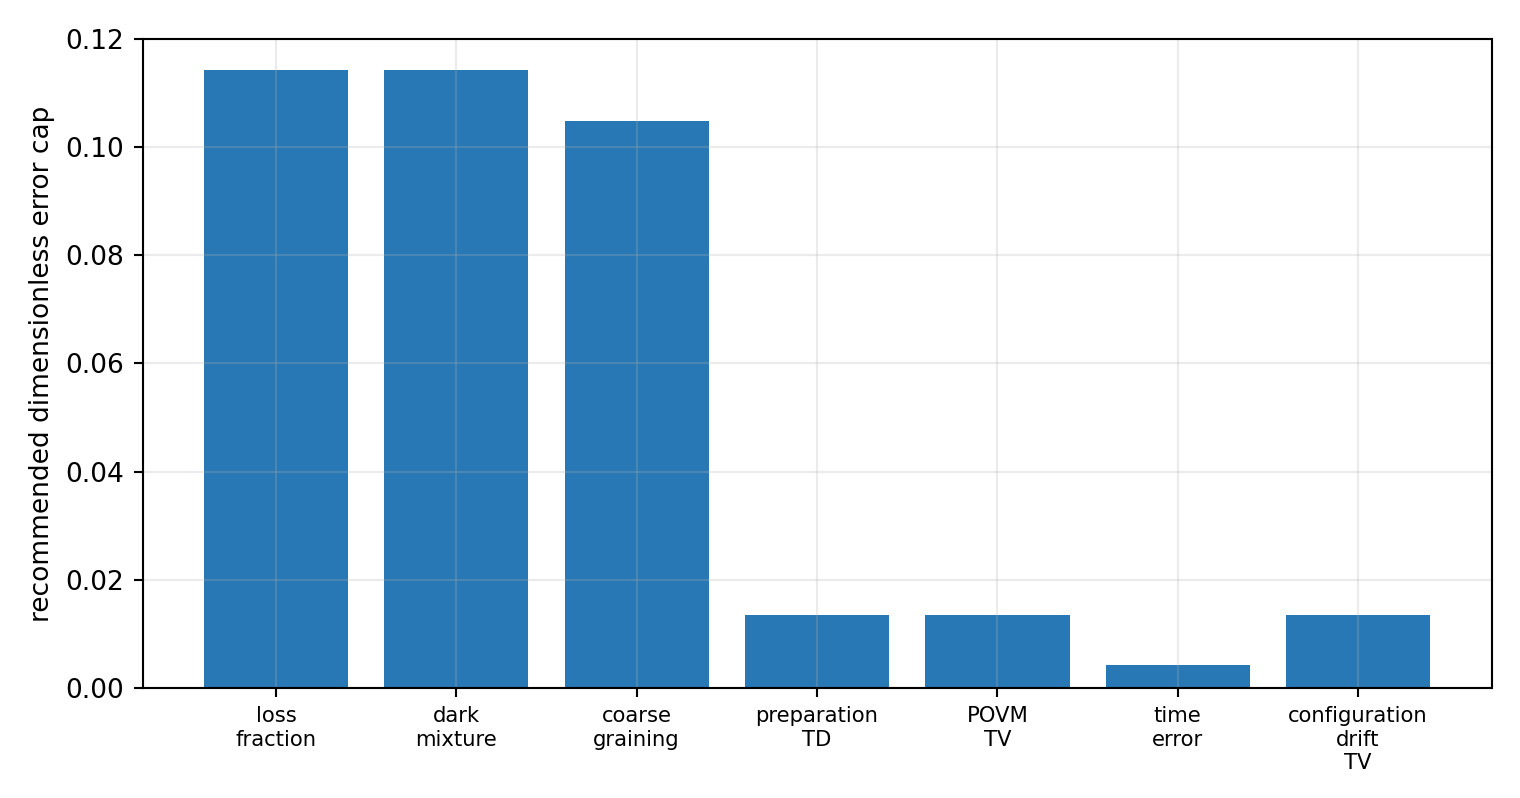
\includegraphics[width=0.82\textwidth]{FIN_Programs_527_536_Figures/p535_inverse_detector_caps.png}
\caption{Synthetic inverse specifications, not measured apparatus tolerances.}
\end{figure}

\textbf{Physical boundary.} P535 does not prove that any laboratory realizes the twelve-state preparation family, vertex POVM, homogeneous FIN semigroup or independent record. It is an executable mathematical target for later experimental design.

\section{P536 --- finite laws are posterior fibers}

Let $R$ evaluate a smooth parameter path at finitely many train and hold-out times $T$. Define
\[
 b(t)=\prod_{\tau\in T}(t-\tau).
\]
For every fitted path $p$, direction $v$ and scalar $c$,
\[
 R[p+c,b,v]=R[p].
\]
Thus any likelihood based only on the finite record is constant in $c$.

\begin{theorem}[Prior-fiber nonidentifiability]
Conditional on all parameters transverse to the vanishing-bump fiber, the posterior distribution of $c$ equals its prior conditional distribution. No Bayesian prior, MDL penalty, Sobolev regularizer or analyticity preference can convert finite records into prior-free identification of an unrestricted off-record law.
\end{theorem}

The numerical ledger illustrates rather than proves the theorem: hold-out-only and a weak Sobolev-like criterion select degree three, whereas BIC-like and stronger complexity penalties select degree two. The invariant output is the quotient class modulo $\ker R$, not one privileged representative.

Future local searches should therefore state the admissible law class before fitting, report at least two inequivalent regularizers, and identify which conclusions are invariant across their selected representatives.

\section{Integrated interpretation after falsification}

The ten studies support the following hierarchy.

\begin{enumerate}
\item \textbf{Quadratic strict core.} The finite self-adjoint graph generator, spectral measure, unitary flow and heat flow remain mathematically secure.
\item \textbf{Nonlinear persistence.} The localized DNLS branch and its favourable stability sector are certified only after an attractive response is supplied.
\item \textbf{Minimal response mechanism.} A positive mediator coupled to information density forces the correct sign by a Schur complement. This is the most economical current candidate for the missing fourth-order source.
\item \textbf{Temporal nonuniqueness.} Eliminating a mediator statically loses essential kinetic information. The same static operator has inequivalent relaxation and Hamiltonian temporal completions.
\item \textbf{Intrinsic time.} Six rationally independent phases supply quasiperiodic internal order and recurrence, but the global scale orbit forbids an absolute clock without new data.
\item \textbf{Operational boundary.} Synthetic separability can be converted into explicit detector budgets and event schemas; it is still not a physical realization.
\item \textbf{Law boundary.} Finite local computation can reject and compare declared law families, but it cannot select an unrestricted law independently of prior structure.
\end{enumerate}

The most defensible current mathematical interpretation remains a finite spectral-adaptive operator framework with a conditional nonlinear mediator completion. It is not yet a physical theory because no theorem selects the mediator from the strict core, sets its dimensional coefficients, resolves orientation, or maps the operational variables to an independently recorded apparatus.

\section{Failed or bounded approaches}

\begin{itemize}
\item Generic entropy/Fisher/compression labels still do not source the focusing sign; P527 succeeds only by adding a mediator premise.
\item Stationary memory persistence does not imply temporal stability; P530 supplies inequivalent realizations.
\item The scanned phase-kick family does not generate a localized relative periodic orbit.
\item Six-frequency recurrence does not generate seconds or energy units.
\item Independent PSD agreement does not make the homotopy a physical process.
\item Detector optimization does not generate calibration, preparation or custody evidence.
\item Hold-out performance and priors do not select an unrestricted evolution law.
\end{itemize}

\section{Recommended local programs P537--P548}

All studies below are executable analytically or on modest local hardware. Priorities reflect probability of producing a proof-grade advance, not importance to a physical narrative.

\begin{longtable}{@{}p{0.08\textwidth}p{0.08\textwidth}p{0.72\textwidth}@{}}
\toprule
ID & Priority & Study and acceptance condition\\
\midrule
P537 & 1 & Construct a bounded saturating mediator potential whose elimination reproduces the P527 quartic jet; prove global coercivity and identify the minimal added coefficient set.\\
P538 & 2 & Interval-enclose P529 nonlinear trajectories in short restart segments; certify a finite-time stable-side tube and unstable-side departure without relying on floating convergence alone.\\
P539 & 3 & Prove or refute Hamiltonian-memory stability with Krein signatures and exact collision conditions.\\
P540 & 4 & Continue the Hamiltonian mediator boundary in $(\varepsilon,\nu)$ and isolate every eigenvalue collision by interval arithmetic.\\
P541 & 5 & Seek a conserved-quantity or resonance obstruction to nonlinear relative-periodic translation; otherwise formulate a validated boundary-value search.\\
P542 & 6 & Use lattice reduction to improve simultaneous six-frequency recurrence, followed by exact phase-residual replay.\\
P543 & 7 & Tighten the Wiener tail and quadrature constants in P533 without changing the kernel or inserting empirical constants.\\
P544 & 8 & Isolate each PSD transition root with an independent rational/Decimal interval Newton certificate.\\
P545 & 9 & Replace the Hoeffding illustration with exact multinomial confidence regions and integer event-count allocation under the P535 half-spaces.\\
P546 & 10 & Classify identifiable finite-dimensional quotients of parameter-law families; report quotient invariants rather than a single prior-selected representative.\\
P547 & 11 & Search current strict artifacts for a typed internal provider of the P527 mediator, explicitly forbidding legacy-role transfer and amplitude inheritance.\\
P548 & 12 & Test whether any genuinely new object from P527--P547 breaks $\operatorname{Aut}(\mathbb Z_{12})$ orientation symmetry. Preserve QW-2191 if none does.\\
\bottomrule
\end{longtable}

\section{Reproducibility and artifact inventory}

The release contains:
\begin{itemize}
\item \texttt{fin\_programs\_527\_536\_research.py} --- complete deterministic generator;
\item \texttt{check\_fin\_p528\_p533\_p534\_certificates.py} --- standard-library certificate replay;
\item \texttt{test\_fin\_programs\_527\_536.py} --- eleven acceptance tests;
\item \texttt{FIN\_Programs\_527\_536\_Results.json} and summary CSV;
\item three machine-readable certificate ledgers and five figures;
\item this source and compiled PDF;
\item the Release 10.53 Zenodo description and SHA-256 manifest.
\end{itemize}

Reproduction commands are:
\begin{verbatim}
MPLCONFIGDIR=/tmp/fin-mpl-1053 python3 fin_programs_527_536_research.py
python3 check_fin_p528_p533_p534_certificates.py
python3 -m unittest -v test_fin_programs_527_536.py
pdflatex -interaction=nonstopmode -halt-on-error \
  FIN_Programs_527_536_Auxiliary_Field_Memory_and_Exact_Replay_Report_EN.tex
sha256sum -c FIN_PROGRAMS_527_536_RELEASE_MANIFEST.sha256
\end{verbatim}

\section{Final conclusion}

The strongest surviving result is narrower and more useful than a claim of physical completion. A minimal auxiliary mathematical object can generate the missing attractive nonlinear sign: a positive mediator linearly coupled to information density and eliminated by a stationary principle. Direct dynamics support the predicted stable and unstable sectors of the resulting finite DNLS. Yet the mediator's kinetic realization matters, and its static elimination cannot choose that realization. Neither the strict spectrum, recurrence torus, PSD phase diagram, detector budget nor finite data selects a dimensional physical law.

Consequently FIN's current frontier is no longer ``find any focusing mechanism.'' One exists and is minimal in a declared class. The frontier is to prove whether FIN itself exports that mediator, its saturation and its scale, while preserving the strict/legacy split and without importing physical interpretation by name. Until that source theorem and an independent operational record exist, the correct status remains a coherent and increasingly well-certified dimensionless operator model with conditional nonlinear and operational completions.

\end{document}
